%!TEX program = xelatex
% 完整编译方法 1 pdflatex -> bibtex -> pdflatex -> pdflatex
% 完整编译方法 2: xelatex -> bibtex -> xelatex -> xelatex
\documentclass[lang=cn,11pt,a4paper,numbers]{elegantpaper}
% \setCJKmainfont[UprightFont = Songti SC Light, BoldFont=Songti SC Bold, ItalicFont=Kaiti SC, BoldItalicFont = Kaiti SC Bold]{Songti SC Regular}
% \setmainfont{Times New Roman}
% \newfontfamily\menlo{Menlo}
\newfontfamily\arial{Arial}
\newcommand{\w}{\boldsymbol w}
\newcommand{\x}{\boldsymbol x}
\newcommand{\g}{\boldsymbol g}
\newcommand{\p}{\boldsymbol p}
\newcommand{\z}{\boldsymbol z}
\newcommand{\intd}{\textrm{d}}
\newcommand{\e}{\textrm{e}}
% \newcommand{\d}{}
\DeclareMathOperator*{\argmax}{arg\,max}
\DeclareMathOperator*{\argmin}{arg\,min}
\usepackage{algorithm}
\usepackage{algorithmic}
\usepackage{tabularx}
\usepackage{multicol}
\usepackage{graphicx}
\usepackage{caption}
\usepackage{url}
\usepackage{amsmath}
% \usepackage{bm}
%%
% \usepackage[T1]{fontenc}
% \usepackage{libertine}
% \usepackage[libertine]{newtxmath}
%%
% \usepackage[T1]{fontenc}
% \usepackage{Alegreya}
%%
% \usepackage[T1]{fontenc}
% \usepackage[urw-garamond]{mathdesign}
%
\usepackage{newtxtext}
\usepackage{newtxmath}
% \usepackage{mathspec}
% \setmainfont{Times New Roman}
% \setmathsfont{Times New Roman}

% \usepackage{bm}


\title{信道编码大作业实验报告}
\author{\kaishu\zihao{5} 夏智康$^\mathcal{a}$\quad 刘祥$^\mathcal{x}$\quad 芦迪$^\mathcal{y}$\quad 吴舒登$^\mathcal{z}$}
% \linespread{2}
% \linebreak
% \newline
\institute{清华大学深圳国际研究生院 信息科学与技术学部,深计研19班\\
$\mathcal{a}$ 2019211193\quad $\mathcal{x}$ 2019211165\quad $\mathcal{y}$ 2019211174\quad $\mathcal{z}$ 2019211167}
% \linespread{3}

% \institute{\href{https://elegantlatex.org/}{Elegant\LaTeX{} 项目组}}

% 不需要版本信息,直接注释即可
% \version{0.07}
% 不需要时间信息的话,需要把 \today 删除。
\date{}

\begin{document}

\maketitle

% \begin{abstract}
% 本文为 \href{https://github.com/ElegantLaTeX/ElegantPaper/}{ElegantPaper} 的说明文档(中文)。此模板基于 \LaTeX{} 的 article 类,专为工作论文写作而设计。设计这个模板的初衷是让作者不用关心工作论文的格式,专心写作,从而有更加舒适,简便的写作体验。如果你有其他问题、建议或者报告 bug,可以在 \href{https://github.com/ElegantLaTeX/ElegantPaper/issues}{ElegantPaper/issues} 留言。如果你想了解更多由 Elegant\LaTeX{} 项目组设计的模板,请访问 \href{https://github.com/ElegantLaTeX/}{https://github.com/ElegantLaTeX/}。
% \keywords{Elegant\LaTeX{},工作论文,模板}
% \end{abstract}

\section{分工情况}

1. 构造射影平面循环LDPC码。其中,吴舒登主要负责PG-LDPC码的编码工作,芦迪主要负责编写摄影平面循环LDPC码的实验笔记并完成一部分编码工作。

2. 构造基于广义B-J码的准循环LDPC码。夏智康主要负责基于广义B-J码的准循环LDPC码的编码工作,并撰写了实验报告中相应的原理和构造部分。

3. 构造基于循环置换矩阵的Array LDPC码。刘祥主要负责基于循环置换矩阵的Array LDPC码的编码工作,并撰写了实验报告中相应的原理和构造部分。

4. 实现迭代算法,可视化并比较三种编码的分组译码错误概率和比特译码错误概率。芦迪主要负责编码实现迭代算法并可视化实验结果,吴舒登主要负责编写此部分的实验报告并总结实验结果。


\section{构造射影平面循环LDPC码}

基于射影平面构造的循环LDPC码其实就是利用射影平面的点线关联矩阵。考虑在有限域$GF(2^s)$上的$m$维射影平面$PG(m,2^s)$。这个平面包含有$n$个点,其中$\displaystyle{n=(2^{(m+1)s}-1)/(2^s-1)}$。在$PG(m,2^s)$中有$\displaystyle{J=((2^{ms}+\cdots+2^s+1)(2^{(m-1)s}+\cdots+2^s+1))/(2^s+1)}$条直线,每条直线上包含有$2^s+1$个点,每个点上又有$\displaystyle{(2^{ms}-1)/(2^s-1)}$条线交叉。伽罗华域$GF(2^{(m+1)s})$是有限域$GF(2^s)$的扩展,且可以看做是射影平面$PG(m,2^s)$的一个实现。令$\alpha$为$GF(2^{(m+1)s})$的本原元,则$GF(2^{(m+1)s})$中的非零元素$\alpha^0,\alpha^1,\cdots,\alpha^{n-1}$组成了射影平面$PG(m,2^s)$中的点。设$\alpha^i,\alpha^j$是射影平面$PG(m,2^s)$中的两个线性独立的点,那么下面点的集合$\{\alpha^i+\beta\alpha^j:\beta\in GF(2^s)\}$就是$PG(m,2^s)$里通过点$\alpha^i$的一条线。两条线没有交点就是平行的,如果有交点也只能有一个交点。

令$PG(m,2^s)$中直线的关联矢量作为矩阵$\boldsymbol{H}_{PG}^{(1)}(m,0,s)$的行,射影平面$PG(m,2^s)$中的点对应于$\boldsymbol{H}_{PG}^{(1)}(m,0,s)$的列。$\boldsymbol{H}_{PG}^{(1)}(m,0,s)$行重为$\rho=2^s+1$,列重为$\displaystyle{\gamma=(2^{ms}-1)/(2^s-1)}$,密度为$\displaystyle{r=(2^{2s}-1)/(2^{(m+1)s}-1)}$。对$m\geq 2,s\geq 2$,$r$非常小,因此$\boldsymbol{H}_{PG}^{(1)}(m,0,s)$是一个低密度矩阵。它的零空间给出了一个长度为$n$的LDPC码$\boldsymbol{C}_{PG}^{(1)}(m,0,s)$,其最小距离至少为$(2^{ms}-1)/(2^s-1)+1$。校验位长度为$n-k=1+(C_{m+1}^m)^s$。

实验要求构造 $q=32, n=q^2+q+1=1057$ 的 PG-LDPC 码。构造过程如下:
\begin{enumerate}[1)]
    \item 由 $\displaystyle{q=2^s, n=(2^{(m+1)s}-1)/(2^s-1)}$ 得$m=2,s=5$,即要考虑有限域$GF(2^5)$上的2维射影平面$PG(2,2^5)$。$PG(2,2^5)$中的点是用$GF(2^{(m+1)s})=GF(2^{15})$中的元素表示的,可以先构造伽罗华域$GF(2^{15})$。$GF(2^{15})$是由本原多项式$p(x)=x^{15}+x^{14}+x^{13}+x^{12}+x^{11}+x^5+x^4+x^3+x^2+x^1+1$生成的。由此,我们可以得到$GF(2^{15})$。
    \item 令$\alpha$为$GF(2^{15})$的一个本原元。令$\beta=\alpha^n$,则$\beta$的阶为$2^s-1$,$\{0,1,\beta,\beta^2,\cdots,\beta^{2^s-2}\}$可以构成$GF(2^5)$。令$\Gamma = \{\alpha^0,\alpha^1,\alpha^2,\cdots,\alpha^{n-1}\}$,则$\{\alpha^i,\beta\alpha^i,\beta^2\alpha^i,\cdots,\beta^{2^s-2}\alpha^i\}$可将$GF(2^{15})$划分为$n$个不相交的子集。
    \item 需要求出经过某一点的任意一条不过原点的直线上的所有其他点。取$PG(2,2^5)$中的任意不同的两个点$\alpha^i,\alpha^j$,则通过这两个点的直线由$\{\eta_1\alpha^i+\eta_2\alpha^j\}$这样形式的点组成,且有$2^s+1$即33个不同的点,只需选择$\eta_1$与$\eta_2$,使得$(\eta_1,\eta_2)$不是另一个选择$(\eta_1',\eta_2')$的倍数即可。简单起见,我们取$i=0,j=1$,那么$\alpha^i=1,\alpha^j=\alpha$。最终得到含有33个点的一条直线。
    \item 得到直线后,由该直线求其关联矢量。该矢量由$n=1057$个点组成。如果某点在直线上,则关联矢量该点处值为1,否则为0.由所得的关联矢量作为校验矩阵的第一行,对该矢量向右循环移位1056次,每次得到的矢量均作为校验矩阵的一行。校验位数目为$1+(C_3^2)^5=244$,因此信息位的数目位813。校验矩阵的大小为$244\times 1057$,这样就得到了长为1057,信息位为813的二维射影平面LDPC码的校验矩阵。
\end{enumerate}

\section{构造基于广义B-J码的准循环LDPC码}
令$GF(q)$表示一个具有$q=2^m$离散元素的伽罗华域。令$[n,k,d]$表示一个码长为$n$,维度为$k$,最小距离为$d$的$q$元线性码。Berlekamp-Justesen(B-J)码是一类长度为$q+1$的MDS码$[q+1,k,q-k+2]$。为了得到围长尽可能大的B-J码,我们仅考虑$q=2^m,k=2$时的情形。可以看出$q$元$[q+1,2,q]$B-J码是$q$元Hamming码$[\frac{q^r-1}{q-1},\frac{q^r-1}{q-1}-r,3]$的对偶码,因此B-J码的生成矩阵就是对应Hamming码的校验矩阵。易知$q$元Hamming码$[\frac{q^r-1}{q-1},\frac{q^r-1}{q-1}-r,3]$的校验矩阵,并将其化为循环形式,就能够得到B-J码的生成矩阵。当$q=32$时,可得$q$元$[33,2,32]$B-J码的生成矩阵为:
\\第一行:$$[1,1,2,3,4,5,6,7,8,9,10,11,12,13,14,15,16,17,18,19,20,21,22,23,24,25,26,27,28,29,30,31,0]$$
第二行:$$[0,1,1,2,3,4,5,6,7,8,9,10,11,12,13,14,15,16,17,18,19,20,21,22,23,24,25,26,27,28,29,30,31]$$
生成多项式为:$$g=(1,1,2,3,4,5,6,7,8,9,10,11,12,13,14,15,16,17,18,19,20,21,22,23,24,25,26,27,28,29,30,31)$$

我们所要构造的基于广义B-J码的准循环LDPC码$q=32,n=q^2-1=1023$。因为码长为$1023=33 \times 31$,所以采用基于B-J码的第二类置换,即$(q-1)$元组置换。

设$C_{B/2}^{*}$为$C_{B/2}$的非0码字集合,由$C_{B/2}$的循环特性易知,$C_{B/2}^{*}$可有如下表示:
\begin{equation}
C_{B/2}^{*} = \{\lambda g(x)x^i: \lambda \neq 0 \in GF(q), i=1,\dots, q+1\}
\end{equation}
令
\begin{equation}
C_i^{(2)} = \{\lambda g(x)x^i: \lambda \neq 0 \in GF(q)\}, \quad i=1,2,\dots, q+1
\end{equation}
易得$|C_i^{(2)}|=q-1$,并且所有的$C_i^{(2)}(i=1,2,\dots,q+1)$构成了$C_{B/2}^{*}$的一个划分。

令矩阵C的行向量为$C_{B/2}^{*}$中的一个码字,同时矩阵C中包含$C_{B/2}^{*}$中的所有码字,易知C为$1023\times 33$矩阵。因为$q$元$[33,2,32]$B-J码是线性等重和等距码,因此所有的非零码字都有着相同的重量32,任意两码字之间的距离也是32,即任意两码字之间至多只有一个分量相同。所以矩阵C中任意两行间只有一个分量相同。对矩阵C中的元素进行$(q-1)$元组替换,即对于$GF(q)$中的非0元素$\alpha^j(j=0,1,\dots,q-2)$,定义一个二元$(q-1)$长向量$\mathbf{y}(\alpha^j)=(y_0,y_1,\dots,y_{q-2})$与$\alpha^j$一一对应,其中$y_j=1$,其他分量为0。而对于$GF(q)$中的0元素则用全0的$(q-1)$长向量与其对应。由此得到的矩阵H为$1023 \times 1023$二元矩阵,而且矩阵H的任意两行之间只有一个对应位置的分量为1,即H的围长大于4。

我们选取$C_{B/2}^{*}$的前6个划分的码字,进行$(q-1)$元组替换得到$186\times 1023$的校验矩阵,对应的LDPC码为$[1023, 837]$。
%令$GF(q^2)$表示$GF(q)$的扩域,并且$\alpha$表示$GF(q^2)$的本原元。由于$q+1|q^2-1$,所以$q$模$q+1$的阶数为2。更进一步,由于$gcd(q,q+1)=1$,不难发现$x^{q+1}-1$可以被完全分解为一个线性因子和许多$GF(q)$上的不同二次方项。令$\beta=\alpha^{q-1}$表示域中的第$q+1$个本原根。对于任意的$i$,不难得到$\beta^{-i}+\beta^i \in GF(q)$。因此,$x^{q+1}-1$的根可以被列为$\beta^{-q/2},\beta^{-q/2+1},\dots,\beta^{-1},\beta^0,\beta^1,\beta^{q/2-1},\beta^{q/2}$,并且
%\begin{equation}
%x^{q+1} - 1 = (x-1)f_1(x)f_2(x)\dots f_{q/2}(x)
%\end{equation}
%其中$f_i(x)=x^2-(\beta^{-i} + \beta^i)x + 1=(x-\beta^{-i})(x - \beta^i)$是在$GF(q)$上的不可约二项式。对于任意的$1<k<q+1$,我们可以构造一个

\section{构造基于循环置换矩阵的Array LDPC}
基于循环置换矩阵的Array LDPC码是一种结构化的LDPC码构造方法,其构造过程主要由三个参数控制$p, j, k$,其中$p$为质数。在这种构造方法下,校验矩阵为
\begin{equation*}
\boldsymbol{H} = 
\begin{bmatrix} 
\boldsymbol{I} & \boldsymbol{I}            &\boldsymbol{I}        & \cdots & \boldsymbol{I} \\
\boldsymbol{I} & \boldsymbol{\alpha}       &\boldsymbol{\alpha}^2 & \cdots & \boldsymbol{\alpha}^{k-1} \\
\boldsymbol{I} & \boldsymbol{\alpha}^2     &\boldsymbol{\alpha}^4 & \cdots & \boldsymbol{\alpha}^{2(k-1)}\\
\vdots         & \vdots                    &\vdots                & \ddots & \vdots \\
\boldsymbol{I} & \boldsymbol{\alpha}^{j-1} &\boldsymbol{\alpha}^{2(j-1)}   & \cdots & \boldsymbol{\alpha}^{(j-1)(k-1)}\\
\end{bmatrix}
\end{equation*}
其中$\boldsymbol{I}$是$p\times p$的单位矩阵,$\boldsymbol{\alpha}$是大小为$p\times p$的左移或右移一位的置换矩阵。例如,当$p=5$时
\begin{equation}
    \boldsymbol{\alpha} = 
    \begin{bmatrix}
        0 & 1 & 0 & 0 & 0 \\
        0 & 0 & 1 & 0 & 0 \\
        0 & 0 & 0 & 1 & 0 \\
        0 & 0 & 0 & 0 & 1 \\
        1 & 0 & 0 & 0 & 0 \\
    \end{bmatrix}
    \text{ 或 }\quad
    \boldsymbol{\alpha} = 
    \begin{bmatrix}
        0 & 0 & 0 & 0 & 1\\
        1 & 0 & 0 & 0 & 0\\
        0 & 1 & 0 & 0 & 0\\
        0 & 0 & 1 & 0 & 0\\
        0 & 0 & 0 & 1 & 0\\
    \end{bmatrix}
\end{equation}
对于题目的要求可取$p=31, k=33, j = 5$,于是信息字长为$k = p\cdot k - p\cdot j = 868$,码长为$n = p \cdot k = 1023$,码率为$k/n=0.8485$。

\section{译码错误概率分析}

使用MATLAB编写了相关程序,实现了前述三种LDPC码的构造,见 \lstinline{./code} 文件夹内的 \lstinline{generate_PG.m}、\lstinline{generate_BJ.m}、\lstinline{generate_Array.m}。其中生成PG-LDPC码的校验矩阵时,需要先运行 \lstinline{./code/pg_ldpc.m} 生成中间变量 \lstinline{GF} 与 \lstinline{points},并将这两个变量作为参数输入 \lstinline{generate_PG} 函数。我们在不同的信噪比下,当检测到10个错误分组,分别计算分组译码错误概率和比特译码错误概率。将分组错误数目除以发送的分组总数目得到分组译码错误概率,使用 MATLAB 中的 \lstinline{berconfint} 函数计算比特译码错误概率。使用MATLAB的通信工具箱(Communication Toolbox)对前面构造的三种LDPC码进行了编解码实验(见 \lstinline{./code/get_BER.m}),并绘制了对应的分组译码错误概率与比特译码错误概率曲线(见 \lstinline{./code/main.m})。

\begin{figure}[htbp]
    \begin{minipage}[t]{0.5\linewidth}
    \centering
    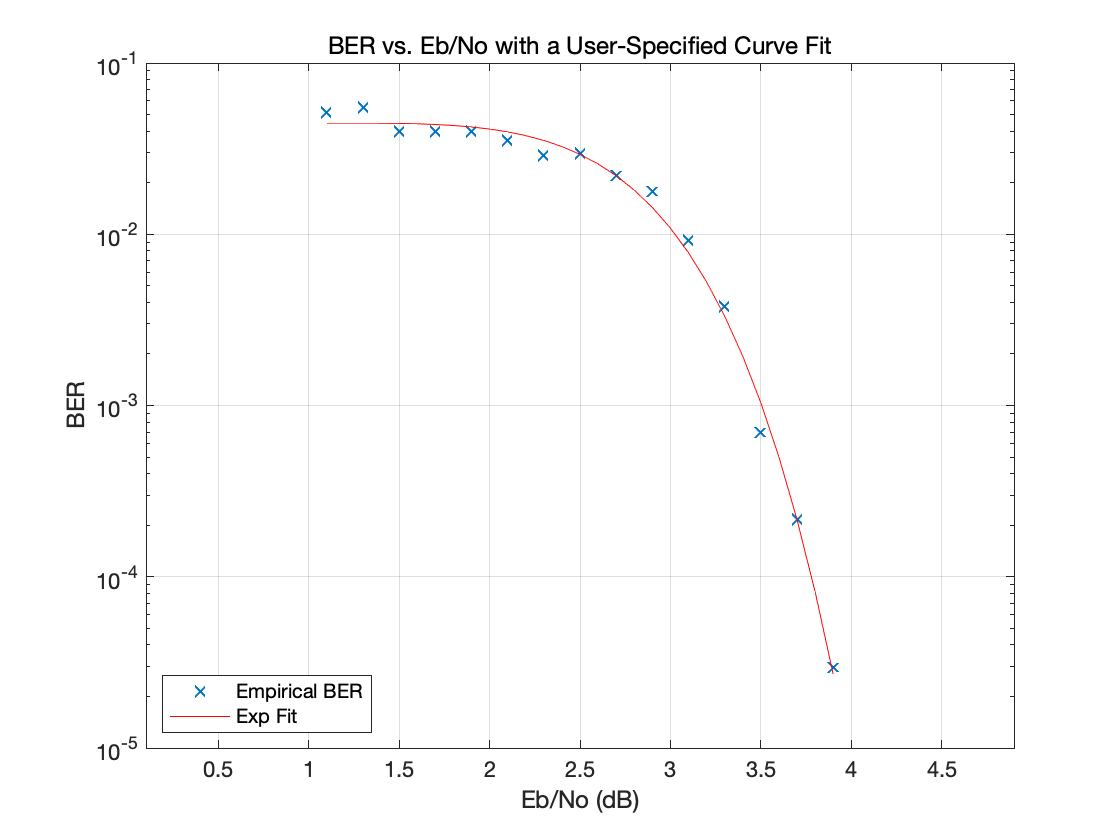
\includegraphics[width=3.1in]{figure/pg_bit_er.png}
    \caption{PG-LDPC Bit Error Rate vs. Eb/No}
    \label{fig:pg_bit_er}
    \end{minipage}%
    \begin{minipage}[t]{0.5\linewidth}
    \centering
    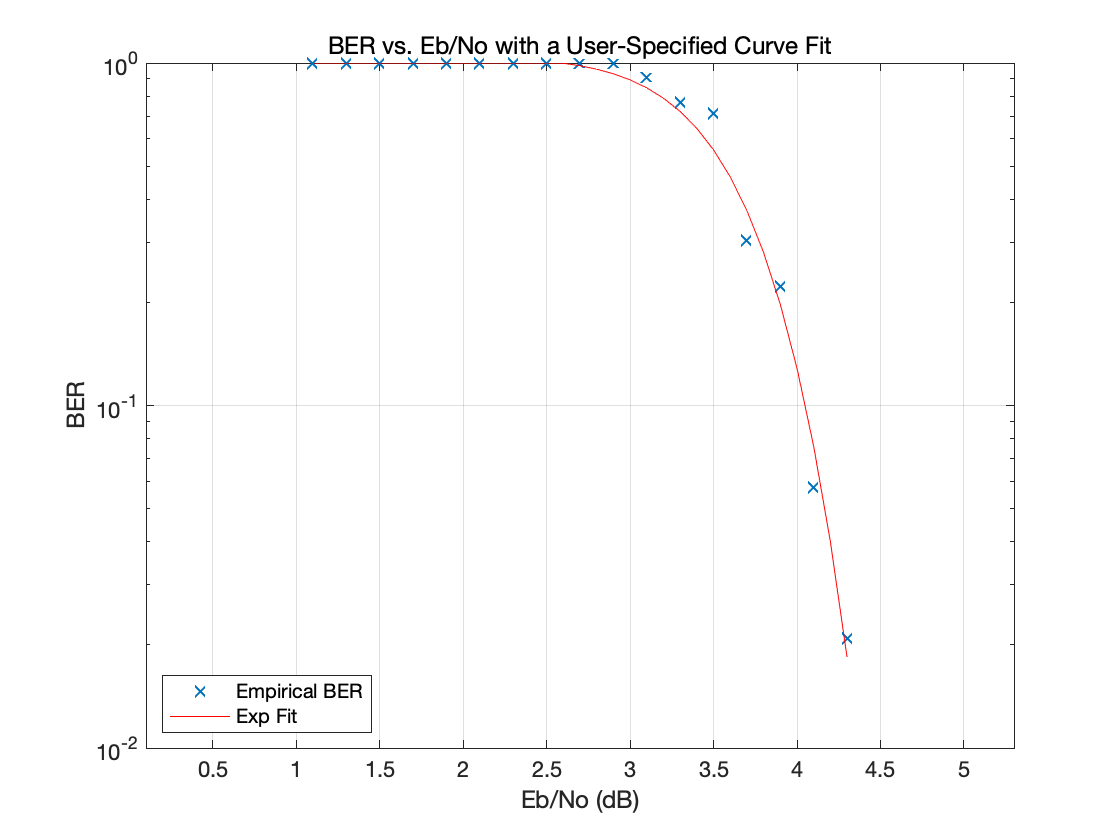
\includegraphics[width=3.1in]{figure/pg_block_er.png}
    \caption{PG-LDPC Block Error Rate vs. Eb/No}
    \label{fig:pg_block_er}
    \end{minipage}
    \end{figure}

\begin{figure}[htbp]
    \begin{minipage}[t]{0.5\linewidth}
    \centering
    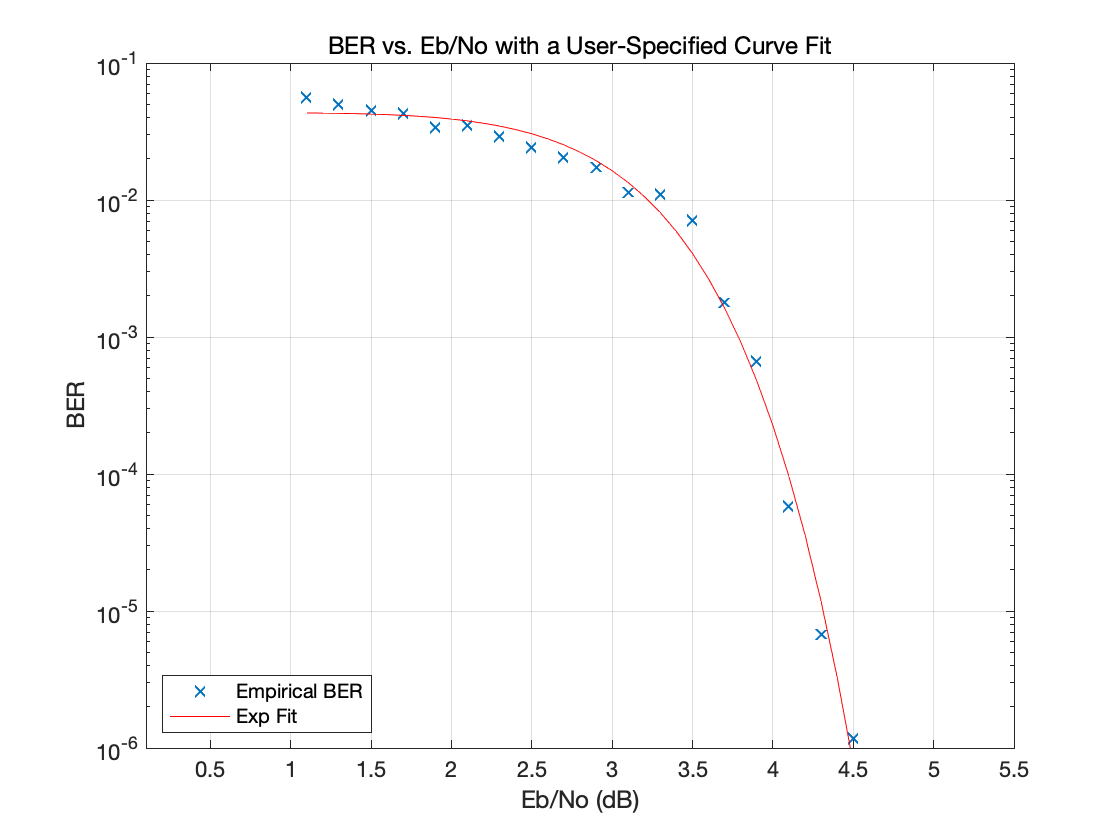
\includegraphics[width=3.1in]{figure/bj_bit_er.png}
    \caption{BJ-LDPC Bit Error Rate vs. Eb/No}
    \label{fig:bj_bit_er}
    \end{minipage}%
    \begin{minipage}[t]{0.5\linewidth}
    \centering
    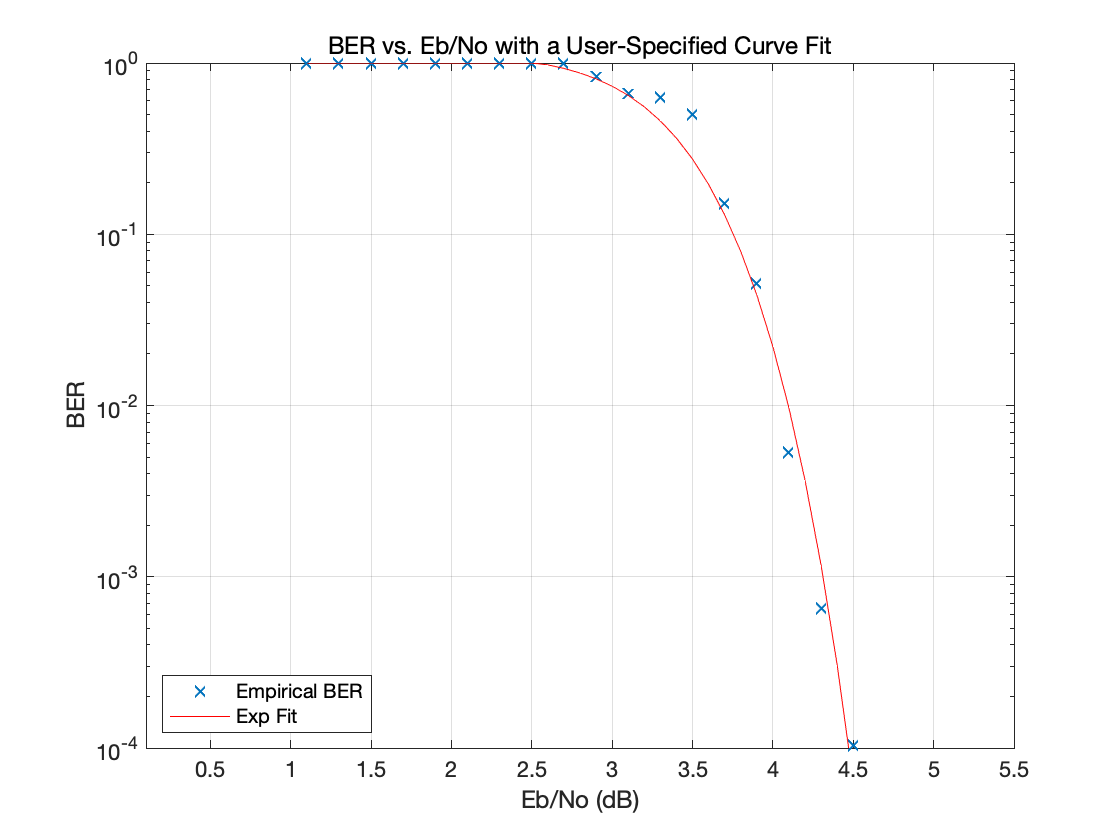
\includegraphics[width=3.1in]{figure/bj_block_er.png}
    \caption{BJ-LDPC Block Error Rate vs. Eb/No}
    \label{fig:bj_block_er}
    \end{minipage}
    \end{figure}

\begin{figure}[htbp]
    \begin{minipage}[t]{0.5\linewidth}
    \centering
    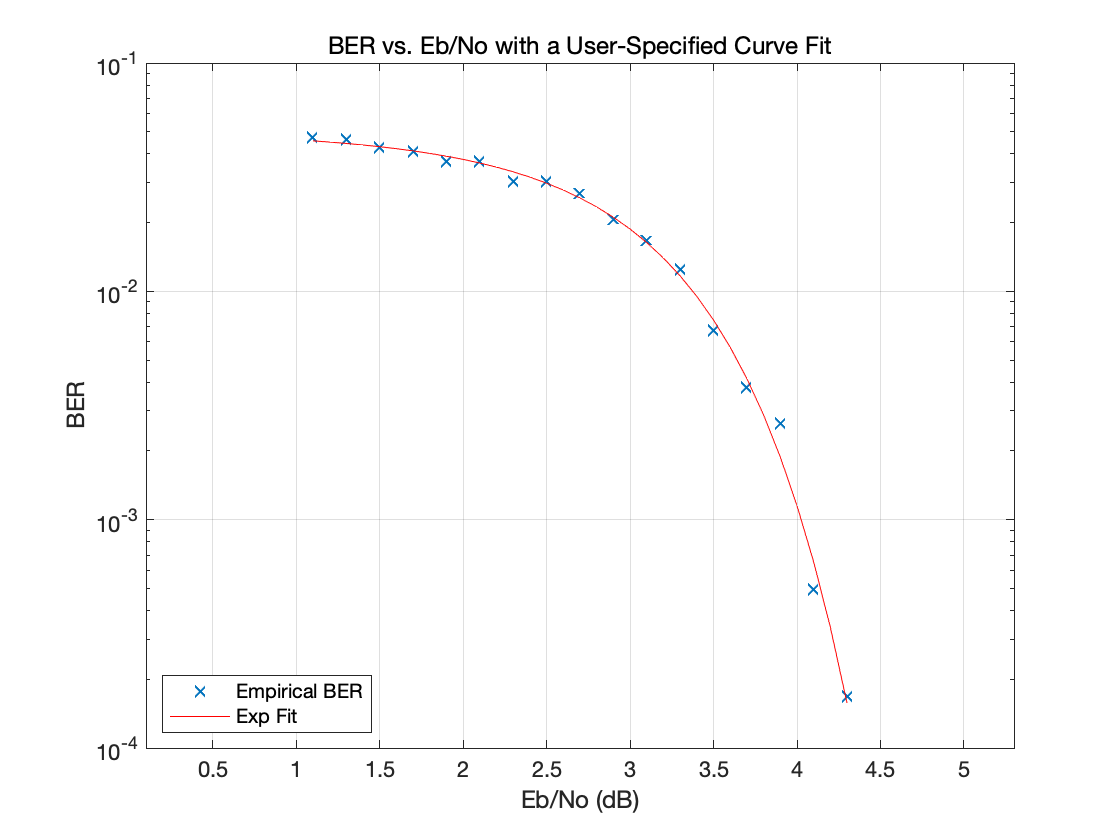
\includegraphics[width=3.1in]{figure/array_bit_er.png}
    \caption{Array-LDPC Bit Error Rate vs. Eb/No}
    \label{fig:array_bit_er}
    \end{minipage}%
    \begin{minipage}[t]{0.5\linewidth}
    \centering
    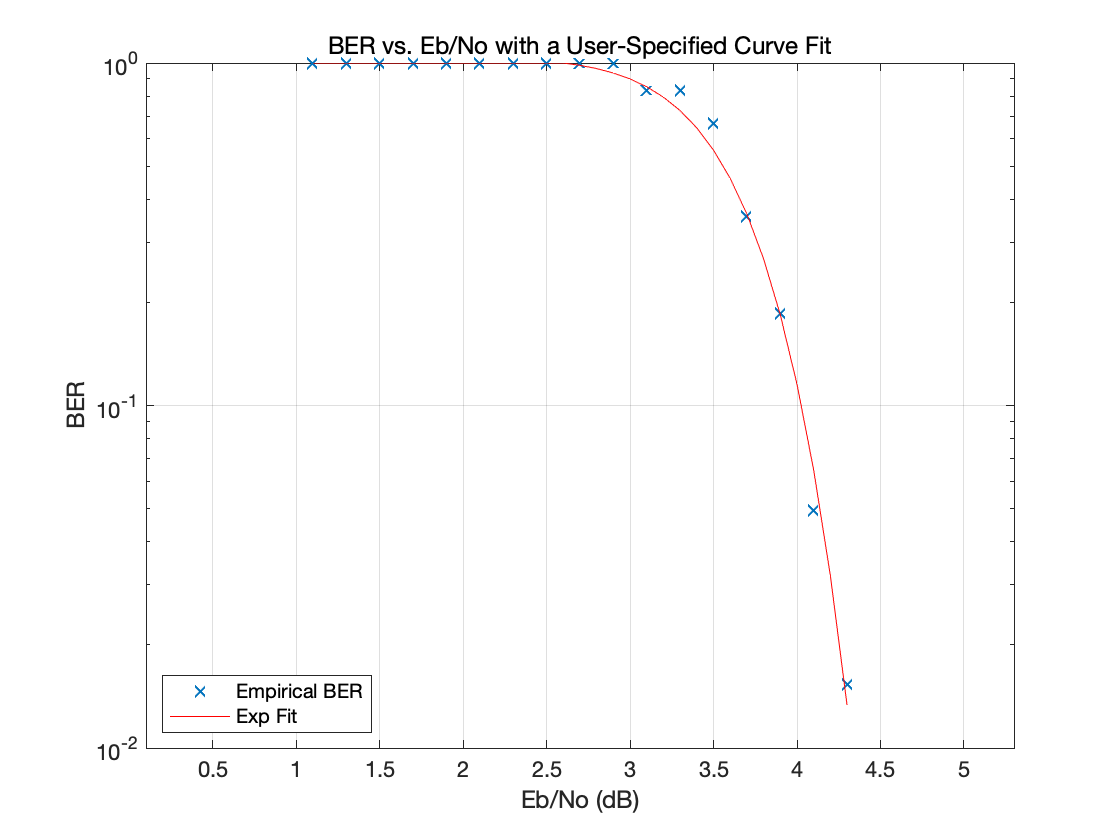
\includegraphics[width=3.1in]{figure/array_block_er.png}
    \caption{Array-LDPC Block Error Rate vs. Eb/No}
    \label{fig:array_block_er}
    \end{minipage}
    \end{figure}

\figref{fig:pg_bit_er}、\figref{fig:pg_block_er}为PG-LDPC 码的分组译码错误概率与比特译码错误概率曲线。在信噪比小于3 dB时,比特错误译码概率较大,大致在(0.01, 0.1)区间;当信噪比超过3 dB时,比特译码错误概率呈指数级下降趋势。当信噪比小于3 dB时,分组错误译码概率接近1;同样地,当信噪比超过3 dB时,分组译码错误概率呈指数级下降趋势。

\figref{fig:bj_bit_er}、\figref{fig:bj_block_er}为BJ-LDPC 码的分组译码错误概率与比特译码错误概率曲线。\figref{fig:array_bit_er}、\figref{fig:array_block_er}为Array-LDPC 码的分组译码错误概率与比特译码错误概率曲线。BJ-LDPC与Array-LDPC的比特译码错误概率和分组译码错误概率的变换趋势与PG-LDPC的变化趋势基本一致。相比而言, 当信噪比逐渐变大,PG-LDPC的分组译码效果更好,在信噪比为3.8 dB时,其错误概率可以低至 \(10^{-3}\),而其余两种编码错误概率大于\(10^{-2}\)。在比特译码方面,也是 PG-LDPC 效果更好,在信噪比达到3.8 dB时,它的错误概率低于\(10^{-5}\),其余两种编码的错误概率在\(10^{-3}\)左右。


\section{总结}
我们的实验主要分成四个部分。在前三部分,我们使用 MATLAB 分别构造投影平面循环LDPC码,基于广义B-J码的准循环码和基于循环置换矩阵的Array LDPC码。第四部分我们实现迭代译码算法,可视化并比较三种编码的分组译码错误概率和比特译码错误概率。通过比较,我们发现比特译码错误概率一致地低于分组译码错误概率;PG-LDPC码在比特译码错误概率和分组译码错误概率上都表现更优越。

\bibliography{wpref}

\end{document}
